\begin{corrige}{DS2012-1-0001}
  \begin{enumerate}
  \item La fonction $\sin(x^2)$ est paire, parce que $(-x)^2= x^2$ et donc $\sin((-x)^2)=\sin(x^2)$. 

    Une fonction paire non nulle ne peut pas \^etre impaire. 

    La fonction $\sin(x^2)$ n'est pas p\'eriodique : si elle l'\'etait il y aurait $T> 0$ tel que $\sin((x+T)^2) = \sin(x^2)$ pour tout $x$ dans $\eR$. Cela veut dire que, pour tout $x$, $(x+T)^2-x^2$ est un multiple entier de  $2\pi$, parce que la fonction sinus est p\'eriodique de p\'eriode $2\pi$.  Mais alors $T=-x+\sqrt{2k\pi+x^2}$, ce qui est impossible parce que la p\'eriode d'une fonction p\'eriodique ne peut pas d\'ependre de $x$. 

  \item 
    \begin{figure}[ht!]
      \begin{center}
        \subfigure[ $f_1(x)=\sin(2x)$]{
          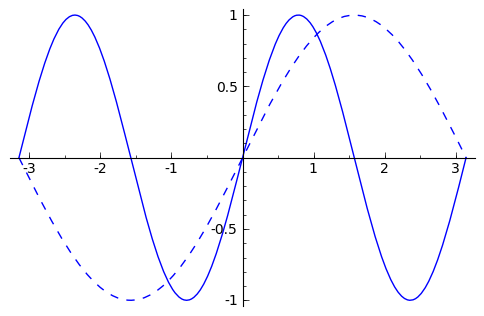
\includegraphics[width=4cm]{sin2x.png}}
        \subfigure[ $f_2(x)=2\sin(x)$]{
          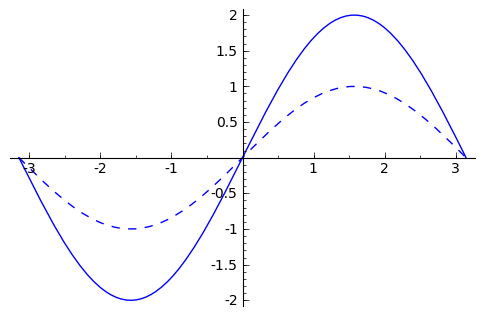
\includegraphics[width=4cm]{2sinx.png}}
        \subfigure[ $f_3(x)=\sin^2(x)$]{
          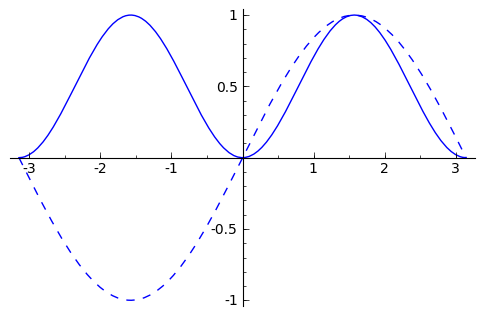
\includegraphics[width=4cm]{sinquadrex.png}}
        \subfigure[ $f_4(x)=\sin(x-1)$]{
          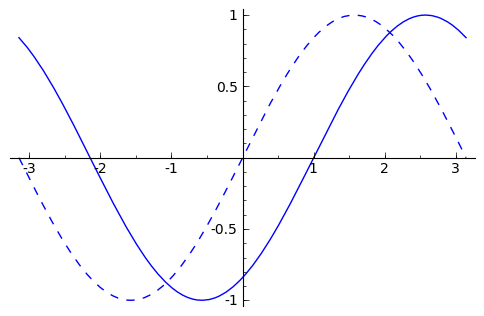
\includegraphics[width=4cm]{sinxmoinsun.png}}
        \subfigure[ $f_5(x)=\sin(x)-1$]{
          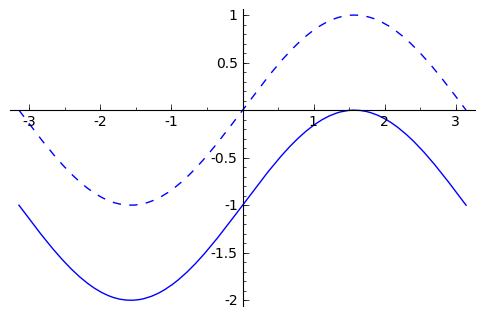
\includegraphics[width=4cm]{moinsunsinx.png}}
      \end{center}
      \caption{Les graphes des fonctions $f_1,\ldots, f_5$}
      
    \end{figure}
    
  \end{enumerate}
\end{corrige}
